\section{Knowledge Needs and Interests? Evidences of Tag Uniqueness and Tag Rank Correlation}
%\textcolor{red}{CCY: Does this section seem too short?}
%\textcolor{blue}{This section is short. I moved it as the first section, so the shortness is less obvious than putting it in between two long sections. Also, the storyline is we first show it is worth to have a non-English site because unique knowledge needs and interests, then we show that do not worry, this will not create community split, and next we show this does create the issues of knowledge fragmentation and duplication, finally this leads to the envision of cross-site retrieval and translation techniques.}
In English Stack Overflow and Russian Stack Overflow, each question can have up to five tags. 
A tag is a word or phrase that describes the topic of the question. 
As a whole, tags used in a Stack Overflow can represent the overall technology landscape that the posts of the site are about~\cite{chen2016techland}.
In this section, we compare the tag usage in ESO and RSO to understand whether and how knowledge needs and interests differ across multi-lingual sites.

\subsection{Tag Rank Correlation}
There are 50,812 tags in English Stack Overflow and 3957 tags in Russian Stack Overflow. 
Among these 3957 tags in Russian Stack Overflow, 821 tags contain Russian characters and the rest 3136 tags are in English. 
We use Google Translate service~\cite{web:googleTranslate} to translate 821 tags with Russian characters into English.

\begin{comment}
However, we can also see that the frequency of a tag may differ between the two sites, for example, \textit{algorithm}(\#58 on ESO, \#21 on RSO), \textit{winforms}(\#69 on ESO, \#29 on RSO), \textit{ruby-on-rails}(\#15 on ESO, \#60 on RSO), etc.
Furthermore, 44 tags, such as \textit{web-application}, \textit{yii2}, \textit{Unity3D}, etc., that appear in the top-100 list of Russian Stack Overflow also exist in English Stack Overflow, but they do not appear in the top-100 list of English Stack Overflow.
Similarly, 44 tags, such as \textit{codeigniter}, \textit{perl}, \textit{maven}, etc.,that appear in the top-100 list of English Stack Overflow also exist in Russian Stack Overflow, but they do not appear in the top-100 list of Russian Stack Overflow.	
\end{comment}

The majority (2560, 64.7\%) of the 3,957 tags in RSO also exist in ESO.
This shows that users of the two sites share much common interest.
Fig.~\ref{fig:tagclouds} shows the word cloud of the top-100 most frequently-used tags in ESO and RSO, respectively.
The font size reflects a tag's relative frequency in its own site, i.e., the larger a tag is, the more frequent it is used in the site.
Among these top 100 frequent tags, 56 of them appear in both sites such as \textit{javascript}, \textit{java}, \textit{C\#}, \textit{android}, etc.
Furthermore, 8 of the top 10 most frequently used tags of RSO are also in the top 10  most frequently used tags of ESO. 
%\textcolor{blue}{CCY: will revise this paragraph later.}
To further understand the interest correlation between two sites, we perform a Spearman Rank Correlation analysis~\cite{zar1998spearman} to 2560 common tags that appear in both sites. 
The Spearman rank correlation coefficient between them is 0.69 ($p-value < 0.005$).
It shows that an implicit increasing monotonic trend between the tag frequency ranks in English Stack Overflow and Russian Stack Overflow. 

We then further analyze tags whose relative frequency in one site is rather different from the other site. 
%\textcolor{red}{CCY: Give some examples that rarely appear in ESO, but relatively frequently appear in RSO. \textbf{And also please conclude several reasons!}}
%\textcolor{orange}{updated at following:}
We first normalize a tag's frequency to a value in (0, 1] through dividing each tag's post number in a site by the total post number of the site.
Fig.~\ref{fig:relfreqbar} shows the comparative ratio of common tags' relative frequency in Russian Stack Overflow to their relative frequency in English Stack Overflow.
The higher (lower) this ratio is, the relatively more (less) frequent a common tag is in Russian Stack Overflow than in English Stack Overflow.
We consider a common tag's relative frequency in the two sites are close if the comparative ratio is within $0.5 < r \leq 2$, i.e., the relative frequencies differ less than twice. 

According to our results, the relative frequencies of 1172 (45.8\%) of 2560 common tags in the two sites are close.
This shows that the level of interests in the technologies these tags represent are not significantly different.
However, the relative frequencies of the rest 1388 common tags differ more than twice.
There are 262 (10.2\%) common tags whose relative frequencies differ more than 10 times, such as \textit{xnet}, \textit{symfony3}, \textit{phpixie}, \textit{vds}, \textit{amazon-web-services}, \textit{android-emulator}, \textit{itext}, \textit{cocoapods}, etc. 
This suggests that the level of interests in these technologies is very different in the two sites.
This interest difference could be caused by many reasons, such as different coding environment, certain technique or tool's popularity in different regions. 
For example, the comparative ratio of the tag \textit{amazon-web-services} is around 0.0063. 
This could be due to the much higher popularity of Amazon web services in English speaking countries than Russia.
%This also suggests that although users of the two sites share much common interest in computer programming techniques, their level of interests in these techniques are different.

\begin{figure}
	\centering
	\subfigure[English Stack Overflow]{
		
\includegraphics[width = 0.48\textwidth]{figures/toptagESO.png}
		\label{fig:ESOtag}}
	\hfill
	\subfigure[Russian Stack Overflow]{  
		
\includegraphics[width = 0.48\textwidth]{figures/toptagRSO.png}
		\label{fig:RSOtag}}
	\caption{Top-100 most frequently used tags in ESO and RSO}
	\label{fig:tagclouds}
\end{figure}

\begin{figure}
	\centering
	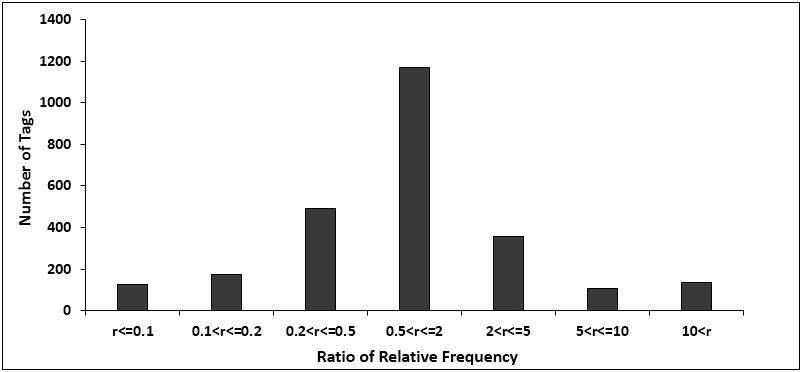
\includegraphics[width = 0.8\textwidth]{figures/relfreqbar.png}
	\caption{Comparative ratios ($r$) distribution of the common tags' relative frequency in RSO to its relative frequency in ESO}
	\centering
	\label{fig:relfreqbar}
\end{figure}

\begin{comment}
\begin{table}
	\small
	\centering
	\caption{Comparative ratios (r) of a common tag's relative frequency on Russian Stack Overflow to its relative frequency on English Stack Overflow \textcolor{blue}{1) use a bar chart. 2) feel that relative frequency ratio differ in 5 times is a too big difference. maybe 2 times is better? if so, split it into $r \leq 0.1$, $0.1 < r \leq 0.2$, $0.2 < r \leq 0.5$, $0.5 < r \leq 2$, $2 < r \leq 5$, $5 < r \leq 10$, $10<r$}}
	\label{tab:rel_freq}
	\begin{tabular}{llllll}
		\hline
		\textbf{r > 10} & \textbf{5 < r <= 10} & $\textbf{1 < r <= 5}$ & $\textbf{0.2 < r <= 1}$ & $\textbf{0.1 < r <= 0.2}$ & $\textbf{ r <= 0.1}$ \\
		\hline
		135 & 105 & 885 & 1135 & 173 & 127 \\
		\hline
	\end{tabular}
\end{table}
\end{comment}


%The tag is a means of connecting experts with questions, and they will be able to answer the question by sorting questions into specific and well-designed categories. 
%Research on the tags is able to reveal a number of most hot fields and topics in the Q\&A website content. 


%To check the overlap and difference of tags between Russian Stack Overflow and Stack Overflow, we first translate Russian tags into English with Google Translate, and then \textcolor{red}{manually revise some incorrect translations ??give some typical examples of such manual corrections?} to make them identical to the main site ones.
\subsection{Tag Uniqueness}
1397 of the 3957 tags in Russian Stack Overflow do not exist in English Stack Overflow.
That is, about 35.3\% technical terms are of interest by only RSO users such as \textbf{Yandx} (the largest Russian search engine in Russia like Google), \textbf{VKontakte} (biggest social network company in Russia like Facebook), \textbf{Denwer} (a popular local server in Russia), \textbf{bitrix} (a popular CMS in Russia written in php), etc.
As these techniques or services that these tags represent are Russian-specific, they are rarely used outside of Russia.
Therefore, ESO does not have questions about these techniques or services.
However, Russian Stack Overflow provides a perfect place to discuss such Russian-specific techniques or services.
These site-specific tags have been used to annotate 61,662 posts in RSO which account for 15.4\% of all 400,185 posts in RSO.

\vspace{2mm}
\noindent \fbox{\centering%
	\parbox{0.98\textwidth}{%		
		\textbf{Summary}:
		According to the tag usage analysis, the majority of tags in RSO are also in ESO.
		However, the level of usage frequency of the common tags often differs between the two sites, which reveals different level of interest in the corresponding technology.
		Furthermore, RSO also has its unique tags whose related posts make an non-negligible proportion of all posts in RSO.
		This shows that non-English speaking users do have unique knowledge needs and interests other than the knowledge in English.
	}%
}
\\

\begin{comment}
	%Ranking the top 10 frequent tags in several sets to show what are the most popular fields in both sites.
\begin{table}[!h]
	\scriptsize
	\centering
	\caption{Top 10 Popular Tags Ranking Statics \textcolor{red}{1) How is freq \% calculated? Need to explain in the discussion. 2) Tags only in Russian should be a separate table. They are not top-10 popular tags.}}
	\label{tab:table4}
	\begin{tabular}{|p{0.8cm}<{\centering}|p{0.55cm}<{\centering}|p{0.8cm}<{\centering}|p{0.55cm}<{\centering}|p{1.5cm}<{\centering}|p{0.55cm}<{\centering}|}
	\hline
	{\scriptsize Main site tags} & freq. (\%) &{\scriptsize Russian site tags} & freq. (\%) &{\scriptsize Tags only in Russian site} & freq. (\%) \\
	\hline
	javascript & 3.39 & php & 6.51  & bootstrap  & 0.304 \\
	\hline
	java & 3.04 & javascript& 5.83  &\bf vkontakte-api & 0.200 \\
	\hline
	c\# & 2.63 & java & 5.31 & android-sdk & 0.178 \\
	\hline
	php & 2.59 & android & 4.43 & android-fragment & 0.143 \\
	\hline    
	android & 2.38 & c\#& 3.89 & mvc & 0.139 \\
	\hline    
	jquery & 2.01 & html & 3.21 & google-maps-api &0.109 \\
	\hline    
	python & 1.87 & jquery& 2.82 & golang & 0.106 \\
	\hline    
	html & 1.59 & c++ & 2.75 & cookie & 0.105 \\
	\hline    
	c++ & 1.23 & css & 2.47  & cms & 0.102 \\
	\hline    
	ios & 1.22 & mysql & 2.08  & \bf yandex-maps-api & 0.092 \\
	\hline 
	\end{tabular}
\end{table}		
\end{comment}

\begin{comment}
\begin{table}[!h]
	\scriptsize
	\centering
	\caption{Different tags preference between two sites \textcolor{red}{why this set of tags as examples? Please tell how do you get this set of tags.} \textcolor{blue}{XINGZC: In addition to showing some examples, I think we need to perform some statistical analysis of the ranks of all 2560 common tags in the two sites, which can show that whether the level of interests in these techniques are statically the same or different.}}
	\label{tab:table_tagpref}
	\begin{tabular}{|l l l l l|}
		\hline
		{\scriptsize Tags} & freq. in SO (\%) & freq. in RSO (\%) & Rank in SO & Rank in RSO \\
		\hline
		web-application & 0.047 & 0.49 & 322  & 32 \\
		\hline
		yii2 & 0.03 & 0.45 & 518  & 35 \\
		\hline
		cuda & 0.029 & 0.012 & 528 & 870 \\
		\hline
		winforms & 0.2 & 0.5 & 63 & 29 \\
		\hline    
		Unity3D & 0.08 & 0.029 & 175 & 58 \\
		\hline    
		website & 0.02 & 0.485 & 734 & 31 \\
		\hline    
		layout & 0.057 & 0.42 & 287 & 41 \\
		\hline    
		Joomla & 0.037 & 0.125 & 424 & 145 \\
		\hline    
	\end{tabular}
\end{table}	
\end{comment}

%According to the result shown in Table~\ref{tab:table4}, it is clear that the most popular areas of two sites are very similar. Though there is some difference among the \textcolor{red}{frequency numbers of the same tag ??you mean absolute frequency number? they are not comparable as the two site are of very different scale, not just due to different preference?} due to the different preference of two sites' users. Overall, 8 of the top 10 most popular tags on Russian site are also the top 10 popular tags on the main site. This indicates that the popular area and content between two sites are highly overlapped. However, focusing on some unique tags in Russian site, it appears some tags who also own considerable frequency. For example, {\bf Yandx}, which is {\bf \foreignlanguage{russian}{Яндекс} }in Russian, is a Russian multinational technology company specializing in search engine and it is the most used search engine in Russia.{\bf []} And {\bf VKontakte}, another Russian local company, is the biggest social network company in Russia and its website, vk.com, is the most popular webstie in Russia.{\bf []} It shows that the Russian sub-site does have some specialness in the content area.